To achieve as high optomechanical coupling as possible it is important to know, where the membrane is in the standing wave inside the cavity. Another important measure is the unmodulated free spectral range denoted by $FSR_0$. This measurement has to be made at cryogenic temperature, as the cavity dimensions are not stable under \SI{300}{\kelvin} $\rightarrow$ \SI{4}{\kelvin} transition, which shifts the cavity resonances.

We obtain these quantities by searching for cavity resonances in the relevant wavelength region, which in our case is \SI{852}{\nano\meter}. We identify the cavity $TEM_{00}$ resonances by use of the camera. We note down the wavelength of the resonance and move on to find the next cavity resonance. Eight resonances is sufficient, but for higher resolution twelve or higher is recommended\footnote{At the same time we do not want to waste precious helium.}. We ended up noting down twelve resonances ranging from \SIrange{850.8}{852.9}{\nano\meter}. We then convert the wavelengths to frequencies and perform a linear fit of cavity resonance frequency as a function of resonance number. The slope of the fit is our $FSR_0 \approx$ \SI{85.0}{\giga\hertz}, corresponding to a cavity length of $L \approx$ \SI{1.77}{\milli\meter}.

We now want to use the transfer matrix model to find at which cavity resonance is the membrane placed closest to a node of the standing cavity wave. To find this point, we subtract the fitted line from the cavity resonance frequencies and assume that the highest frequency value is placed at a node, i.e. zero cavity resonance modulation as in our prediceted model from section \ref{sec:trans_matrix}, which is justified as the membrane inside the cavity can only make cavity length $L$ longer. By using this method we are constantly underestimating the resonance modulation caused by the membrane in the cavity, but this is a small systematic error caused by the relative low resolution, which we do care about since it is just an offset.

To find the membrane position away from the end mirror denoted $\Delta x$ we fit the following model \eqref{eq:resonance_var} to our data. We expect a periodic behaviour modulation in $k$ with period $T_k = \pi/\Delta x$. We ``fold back" the series into the k-range $[0, \pi/\Delta x]$ by sending $k \rightarrow \mathrm{mod}_{\pi}(k\Delta x)$. We end up with the following figure (see \ref{fig:2kz}), showing the cavity resonance frequency modulation as a function of $\mathrm{mod}_{\pi}(k\Delta x)$.

\begin{figure}[H]
\centering
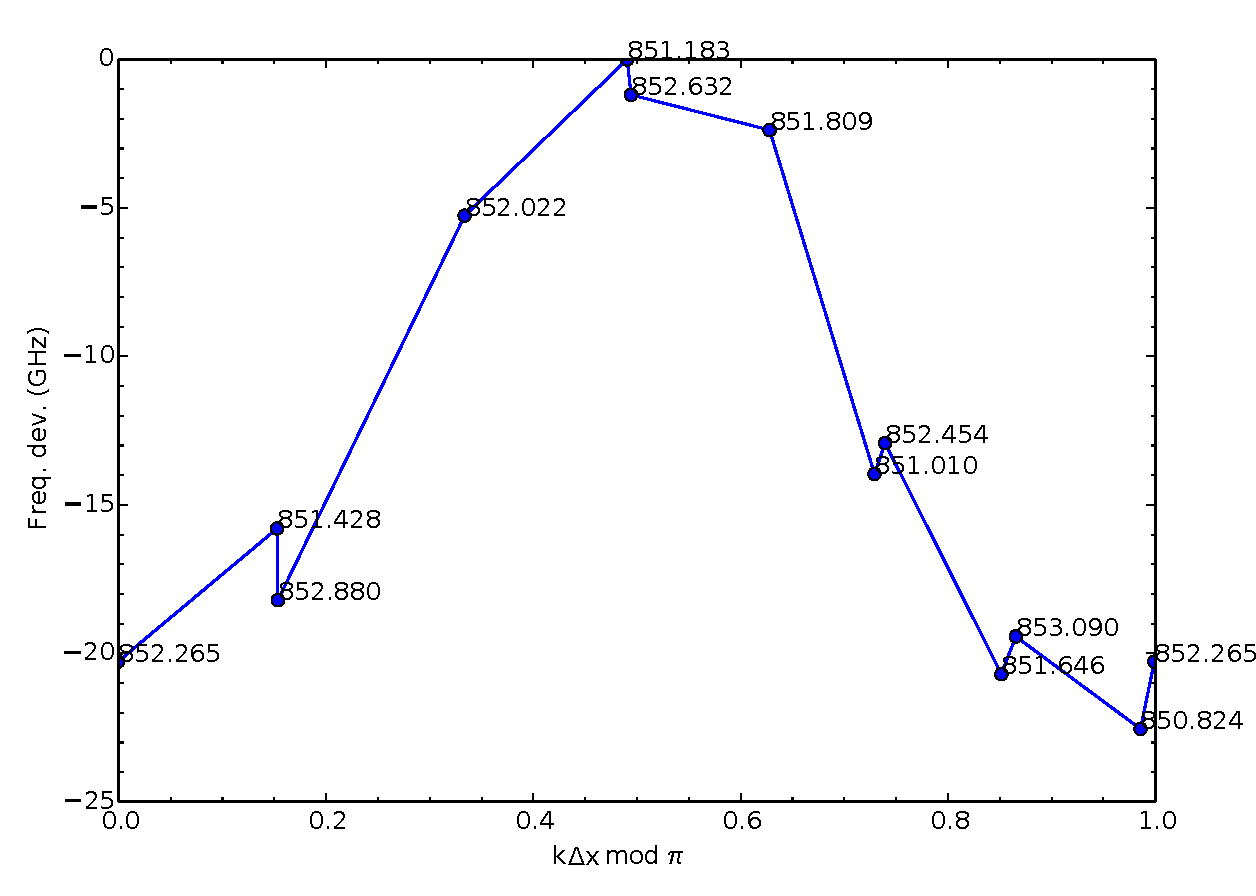
\includegraphics[scale=0.75]{analysis/2kz_mod.pdf}
\caption{Periodicity of the cavity resonance frequency modulation.}
\label{fig:2kz}
\end{figure}

We can now choose a cavity resonance with a high coupling from one of the two slopes of figure \ref{fig:2kz}. But it turns out that experimentally we cannot lock to the cavity resonances on the positive slope, due to what we expect to be a thermal instability. The instability is thought to arise from an asymmetry in the membrane chip geometry, which make it always protrude a little in one direction, causing heating to either push the protrusion towards an unstable region or a stable region depending on position in the standing wave. We can simple state that one slope is stable, while the other is not. We choose our stable cavity resonance coupling point to be at \SI{852.454}{\nano\meter}.

We measure the linewidth for this particular cavity resonance, by scanning the laser frequency across the resonance, while having EOM generating sidebands to calibrate the time axis from the oscilloscope to frequency.

\begin{figure}[H]
\centering
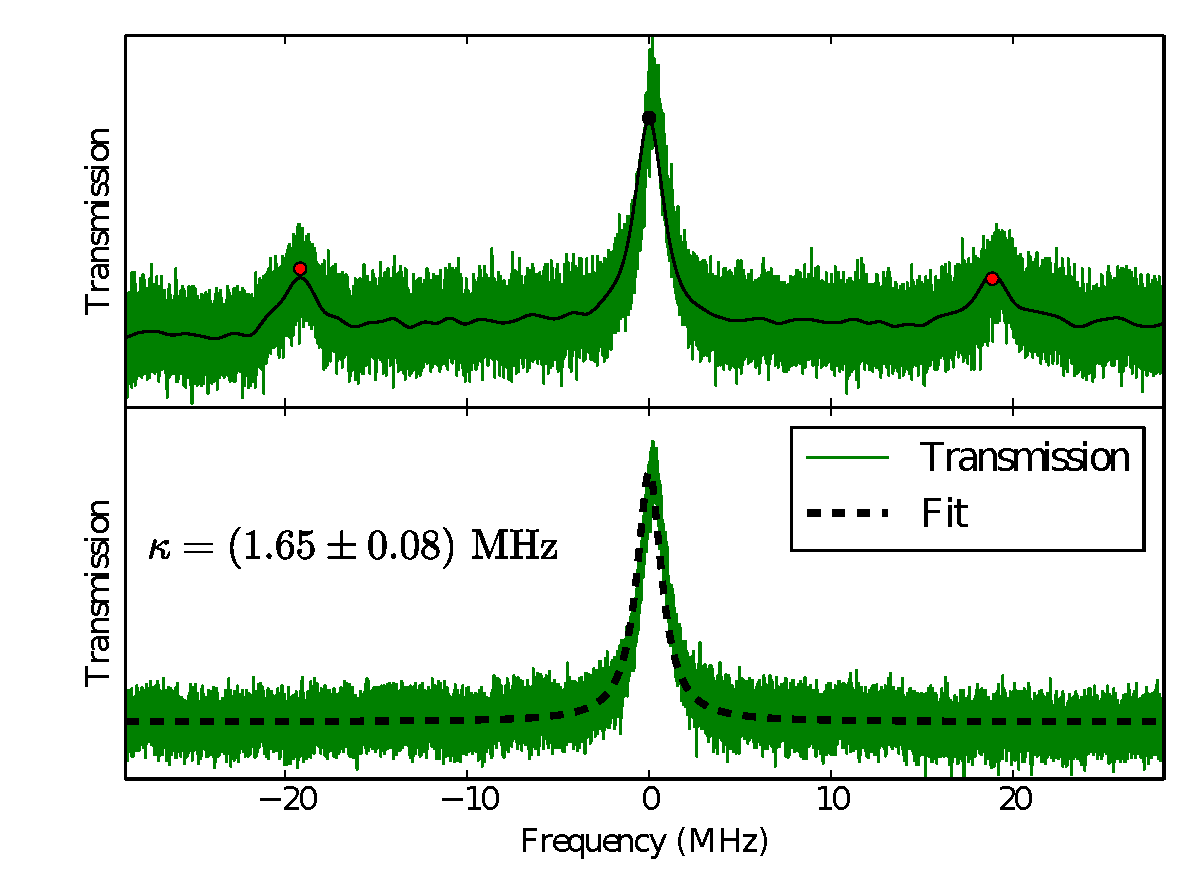
\includegraphics[scale=0.75]{analysis/cav_linewidth.pdf}
\caption{Example of a cavity linewidth measurement. Upper part of the figure show the time trace with sidebands and the lower part show the calibrated to frequency cavity response.}
\label{fig:2kz_cav_lw}
\end{figure}
\noindent
From the three consecutive measured linewidth we get an average of $(1.60 \pm 0.06)$ \SI{}{\mega\hertz}. The increase in cavity linewidth compared to the bare cavity of \SI{0.5}{\mega\hertz} can be assigned to finesse modulation seen from the transfer matrix model \cite{Wilson2011} and not from additional external losses caused by membrane tilt or poor alignment.